%this file is the second report
%a % comment anything after % until the end of the line

%minimum references to begin our article
\documentclass[12pt]{article}
\usepackage[english]{babel}
\usepackage[utf8]{inputenc}
\usepackage[T1]{fontenc}
\usepackage{graphicx}
\usepackage{fancyhdr}
\usepackage{hyperref}
\usepackage{float}
\usepackage{enumitem}
\usepackage{amsmath}
\usepackage[margin=1in]{geometry}
\usepackage{indentfirst}
\usepackage{titlesec}
\usepackage{verbatim}
\usepackage{url}
\usepackage{subfig}
\usepackage{float}
\usepackage{pdfpages}
\usepackage{rotating}
\usepackage{caption}
\newcommand{\sectionbreak}{\clearpage}
\begin{document}
\section{Introduction}	


\subsubsection{Gantt diagram}
\clearpage

\thispagestyle{empty}
\begin{figure}[htb]
\begin{center}
\makebox[\textwidth]{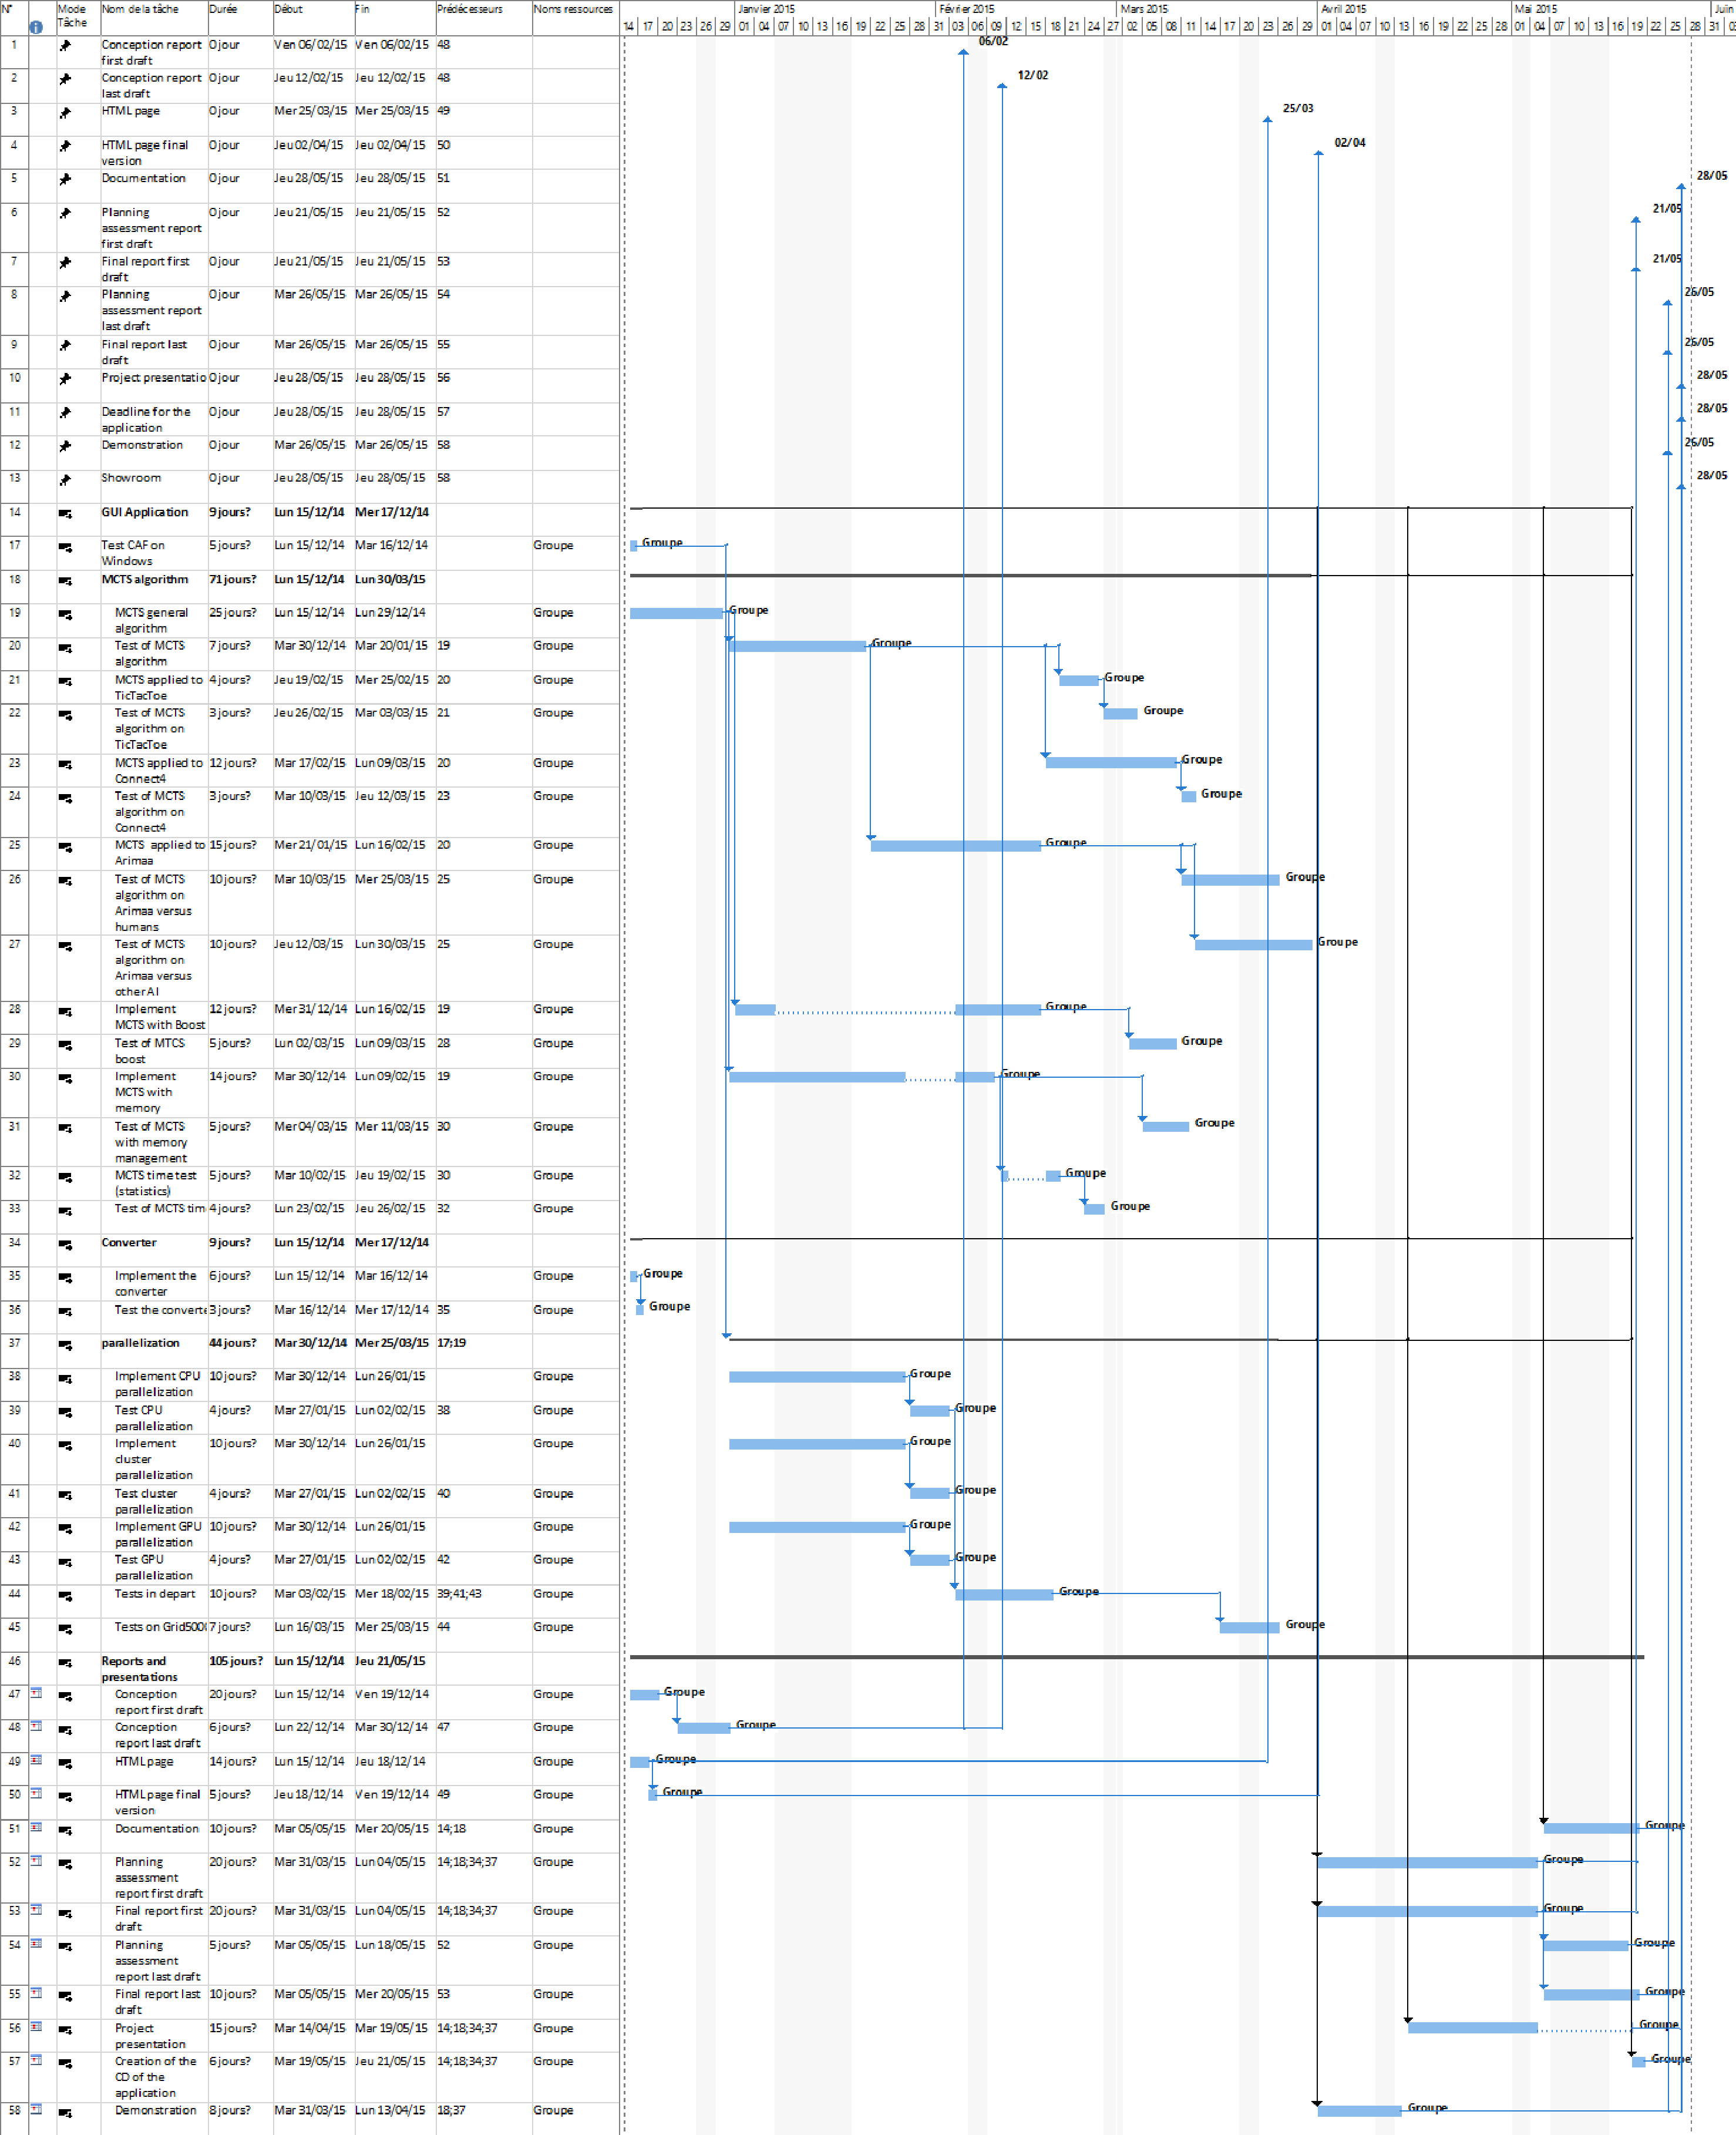
\includegraphics[angle = 90,scale = 0.55,viewport=500 957 1300 1625]{g.pdf}}
\end{center}
\end{figure}
\clearpage

\thispagestyle{empty}
\begin{sidewaysfigure}[htb]
\begin{center}
\makebox[\textwidth]{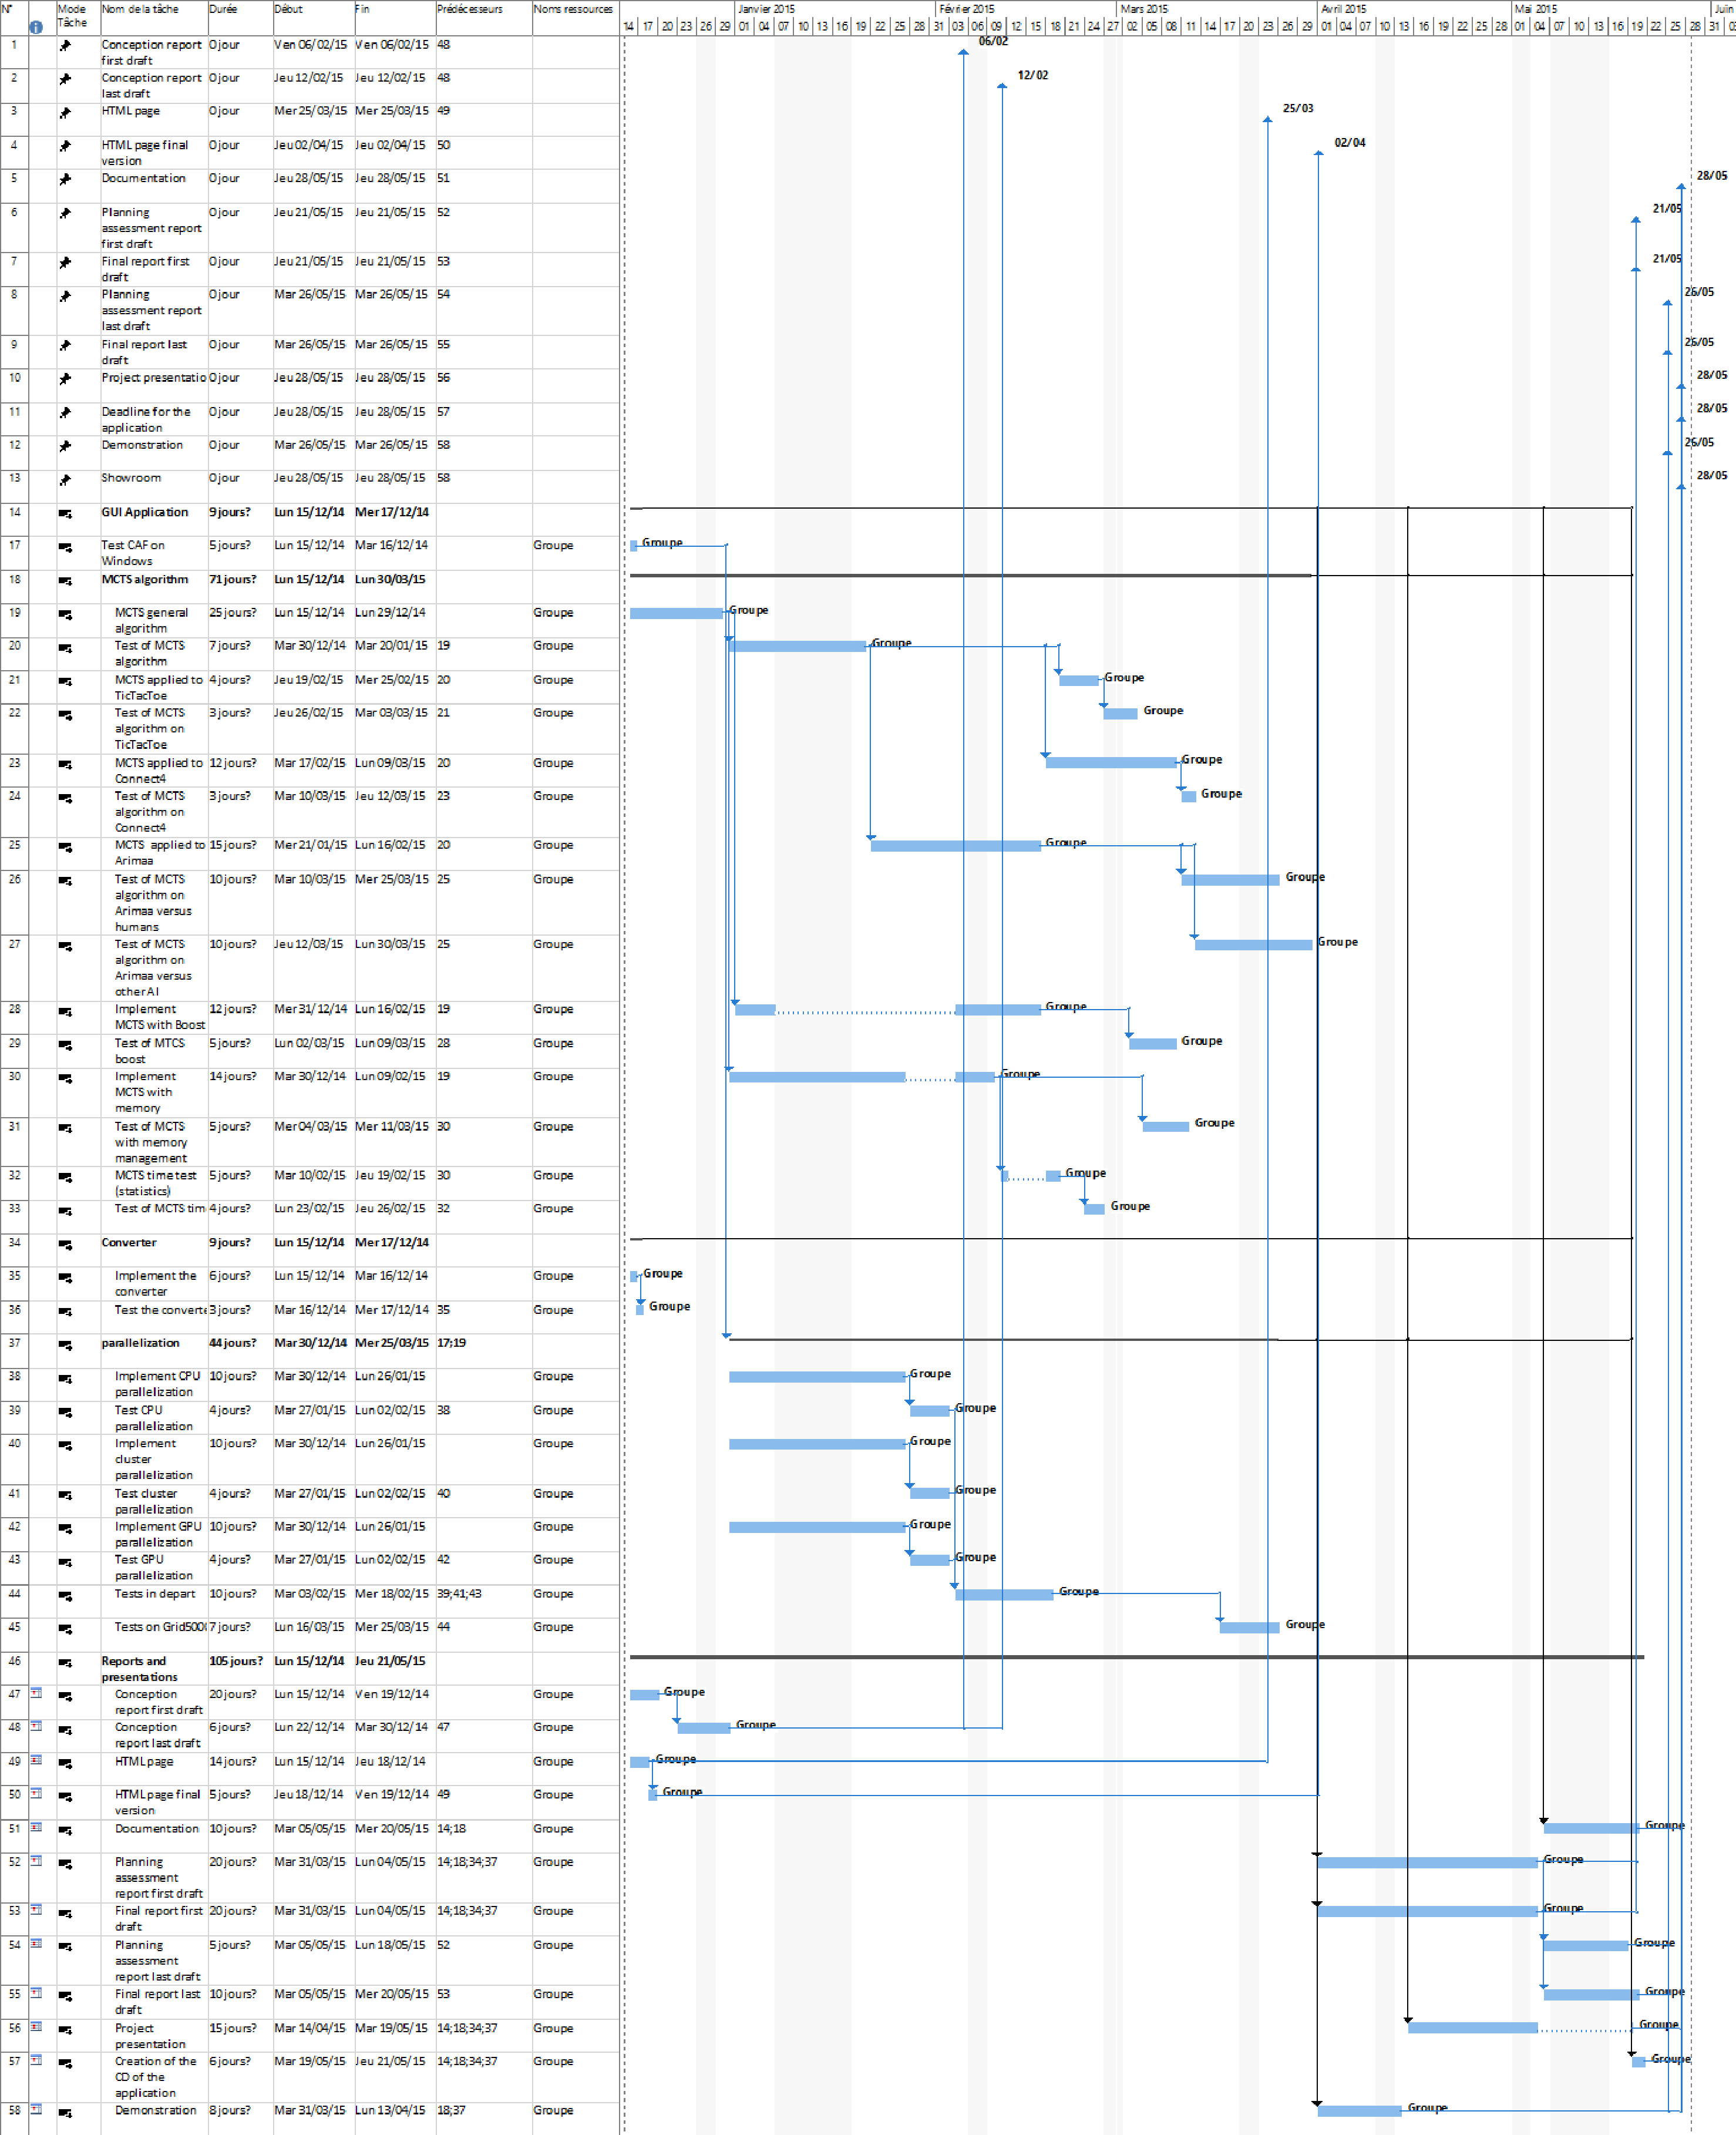
\includegraphics[scale = 0.55,viewport=122 70 1300 370]{g.pdf}}
\caption*{\newline \newline \newline \newline Figure 1 : Gantt Diagram}
\label{fig:ref}
\end{center}
\end{sidewaysfigure}
\clearpage









\clearpage
sdhjfds

\end{document}
